\section{Mobile Technology}

Mobile technology is technology used for cellular communication. \cite{mobileTechnology} After the
rise of smartphones, it has become more and more common to use mobile phones as computers for
anything from reading news to playing games. This section will talk about the mobile platforms the
customer wants us to develop the game for, Android and iOS.

\begin{figure}[!ht]
    \centering
    \subfigure{
    
\includegraphics[scale=0.06]{pictures/android}
    }
    \subfigure{
    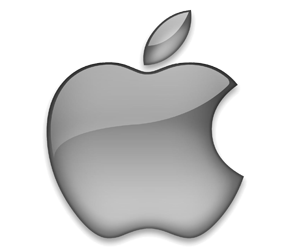
\includegraphics[scale=0.2]{pictures/apple-logo}
    }
    \caption{Android and IOS}
\end{figure}

\subsection{Mobile Platforms}

\subsubsection*{Android}

    Android is a Linux-based operating system, designed for mobile devices with touch screens.
    Android is an open source project primarily being developed by Google and is deployed on various
    mobile devices by third parties.\cite{android} Advantages with developing for Android is that
    development is free. Native applications for Android are developed using Java, which is a well
    known programming language that is taught to everyone studying Computer Science at NTNU. Android
    applications can be developed on both Windows, Mac and Linux so anyone with a computer can
    develop for Android. The Android emulator AVD (Android Virtual Device) means that you don't need
    to own an Android device to test your code. The main disadvantage of developing for Android is
    that there are many devices, running different versions of the operating system, which makes
    testing more demanding.

\subsubsection*{iOS}

    iOS is an operating system developed by Apple primarily for the iPhone, which has been extended
    to run on other Apple devices such as the iPad. Apple does not allow iOS to be deployed on non-
    Apple hardware.\cite{ios} The advantage with developing for iOS is that the number of different
    devices running iOS is smaller and things like screen resolution is more standardized, making
    development and testing easier. The disadvantages are that you have to use Apple hardware and
    software to develop for iOS, distribution of applications for iOS requires a yearly
    subscription\cite{iosCost} and Apple's application store enforces strict terms of distribution
    and requirements that has to be filled in order for your application to get on the application
    store.

\subsection{Conclusion}

    The customer wanted us to develop for both Android and iOS.
    Ultimately it would have made development easier for us if we could select one platform and
    stuck to it, probably Android because of all the advantages it has and because other group
    members have previous experience with developing for Android. However the customer wanted both
    platforms and therefore we agreed to this requirement.
